\documentclass{beamer}
\mode<presentation>
\usetheme{CambridgeUS}
\usepackage[russian]{babel}
\usepackage[utf8]{inputenc}
\usepackage[T2A]{fontenc}
\usepackage{sansmathaccent}

\usepackage{verbatim}
\usepackage{alltt}

\pdfmapfile{+sansmathaccent.map}
\title[Язык C]{Основы программирования на С}
\author{Наумов Д.А., доц. каф. КТ}
\date[10.09.2019] {Операционные системы и системное программное обеспечение, 2020}

\begin{document}

%ТИТУЛЬНЫЙ СЛАЙД
\begin{frame}
  \titlepage
\end{frame}
  
%СОДЕРЖАНИЕ ЛЕКЦИИ
\begin{frame}
  \frametitle{Содержание лекции}
  \tableofcontents  
\end{frame}

\section{Основные операторы языка}

\begin{frame}{Операторы языка С}
\begin{figure}[h]
\centering
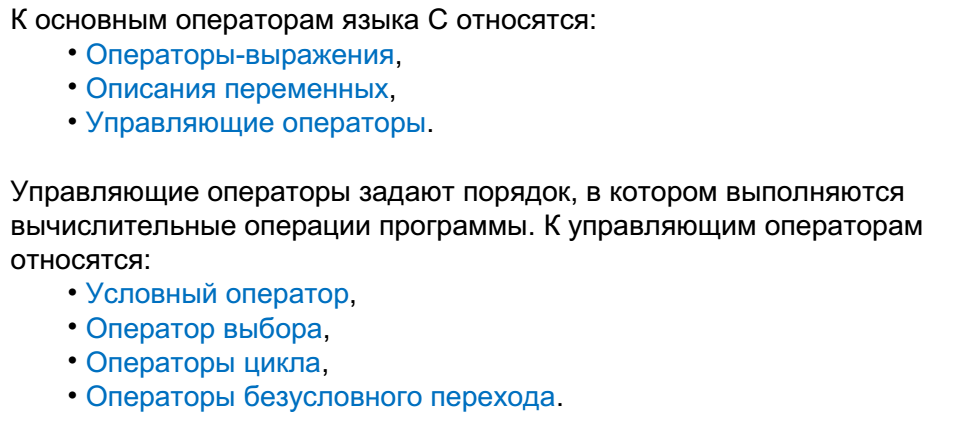
\includegraphics[scale=0.4]{images/lec02-pic01.png}
\end{figure}
\end{frame}

\section{Операторы-выражения}

\begin{frame}{Операторы-выражения}
\begin{figure}[h]
\centering

\includegraphics[scale=0.4]{images/lec02-pic02.png}
\end{figure}
\end{frame}

\begin{frame}{Блоки}
\begin{figure}[h]
\centering
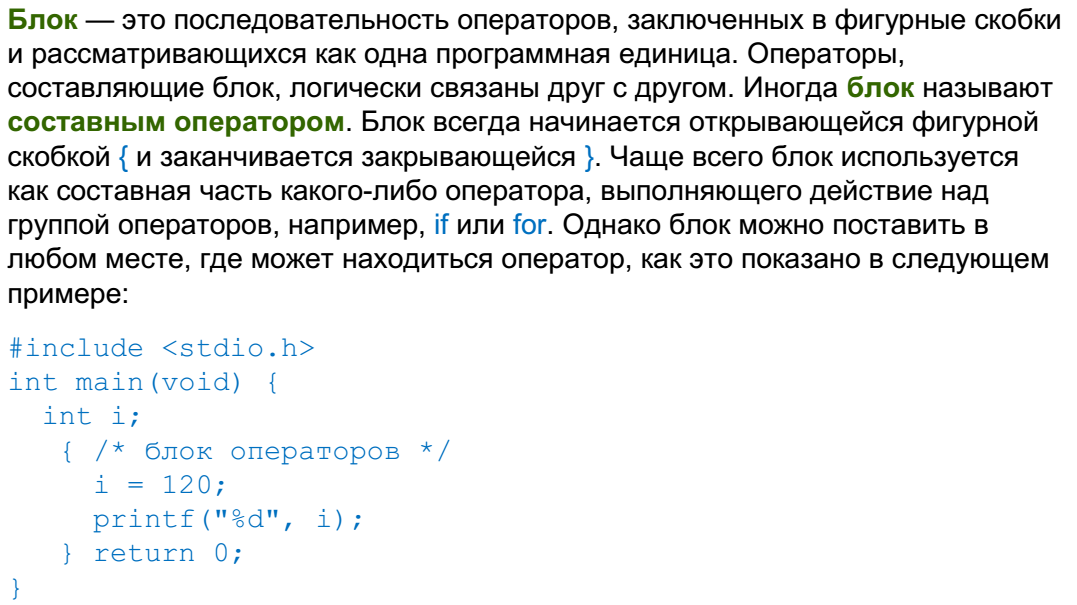
\includegraphics[scale=0.4]{images/lec02-pic03.png}
\end{figure}
\end{frame}

\section{Объявления переменных}

\begin{frame}{Объявления переменных}
\begin{figure}[h]
\centering
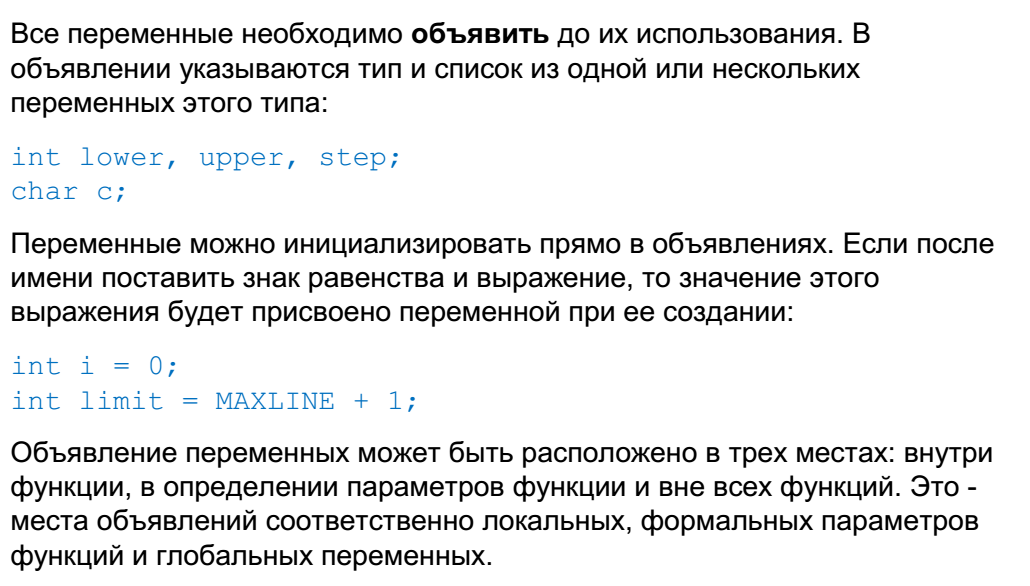
\includegraphics[scale=0.4]{images/lec02-pic04.png}
\end{figure}
\end{frame}

\begin{frame}{Области видимости переменных}
\begin{figure}[h]
\centering
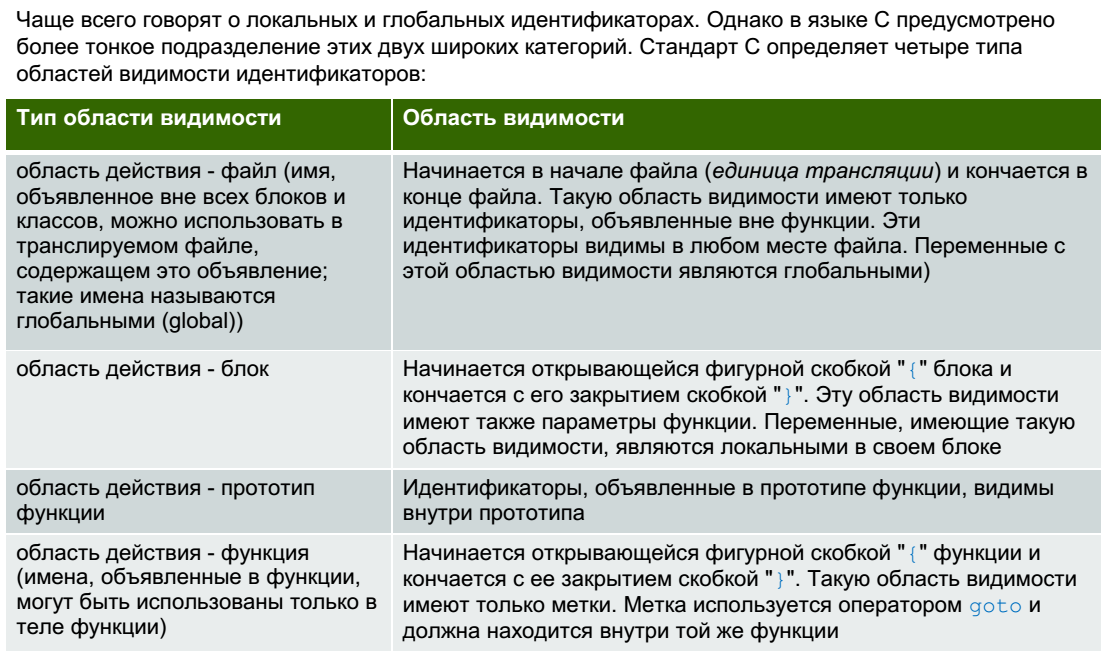
\includegraphics[scale=0.4]{images/lec02-pic05.png}
\end{figure}
\end{frame}

\begin{frame}{Квалификатор типа}
\begin{figure}[h]
\centering

\includegraphics[scale=0.4]{images/lec02-pic06.png}
\end{figure}
\end{frame}

\begin{frame}{Квалификатор const}
\begin{figure}[h]
\centering
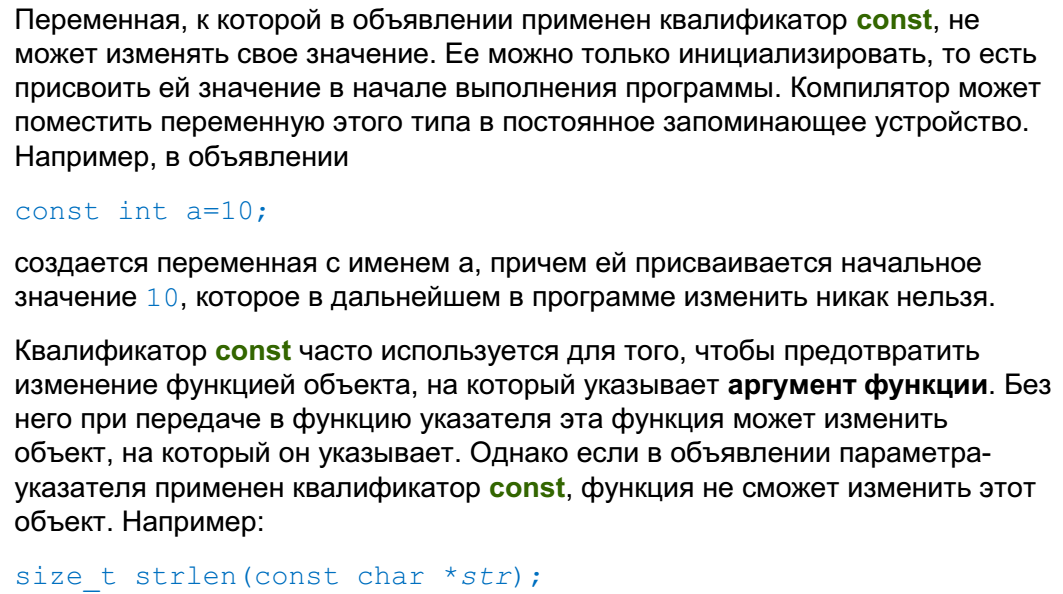
\includegraphics[scale=0.4]{images/lec02-pic07.png}
\end{figure}
\end{frame}

\begin{frame}{Квалификатор volatile}
\begin{figure}[h]
\centering
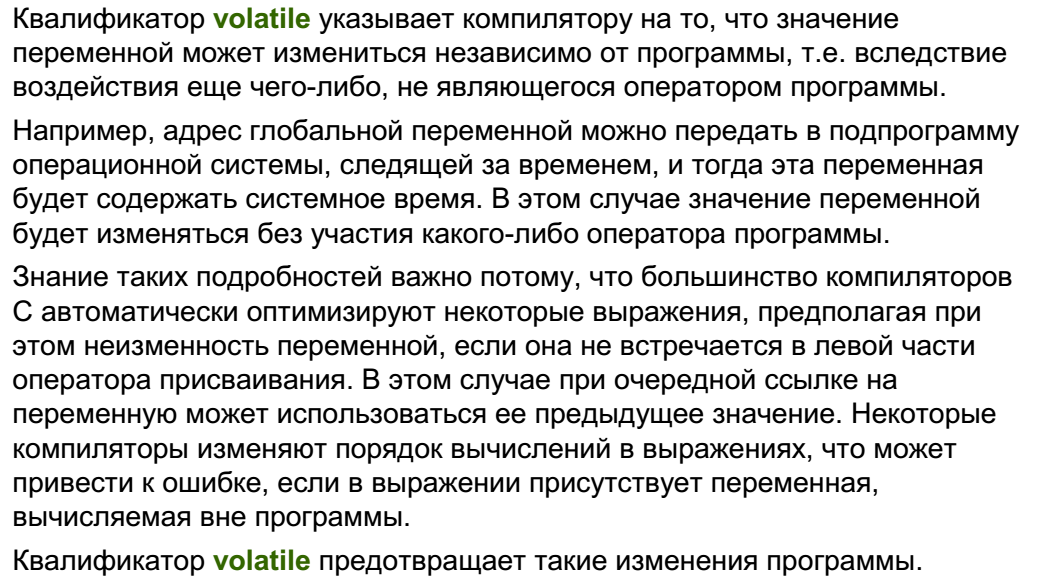
\includegraphics[scale=0.4]{images/lec02-pic08.png}
\end{figure}
\end{frame}

\begin{frame}{Спецификаторы класса памяти}
\begin{figure}[h]
\centering
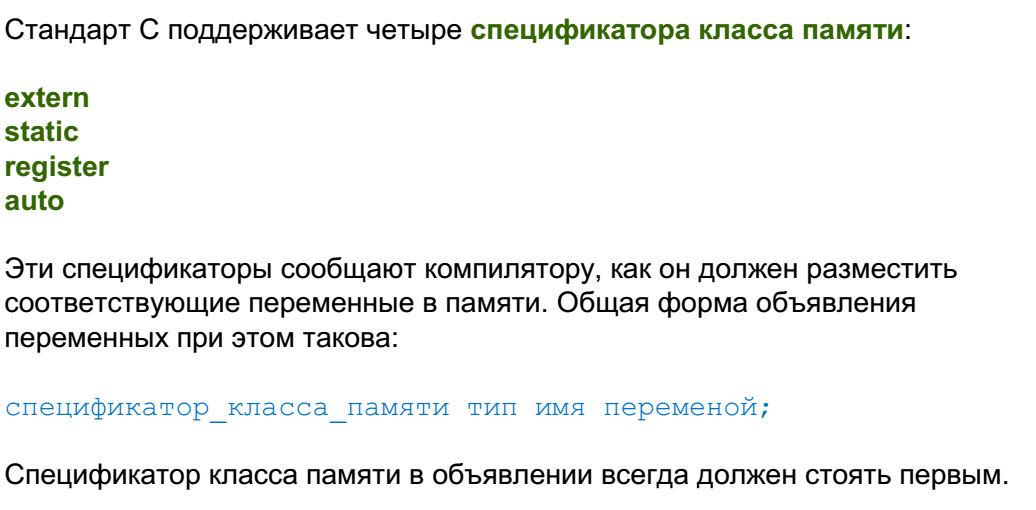
\includegraphics[scale=0.4]{images/lec02-pic09.png}
\end{figure}
\end{frame}

\begin{frame}{Спецификатор extern}
\begin{figure}[h]
\centering
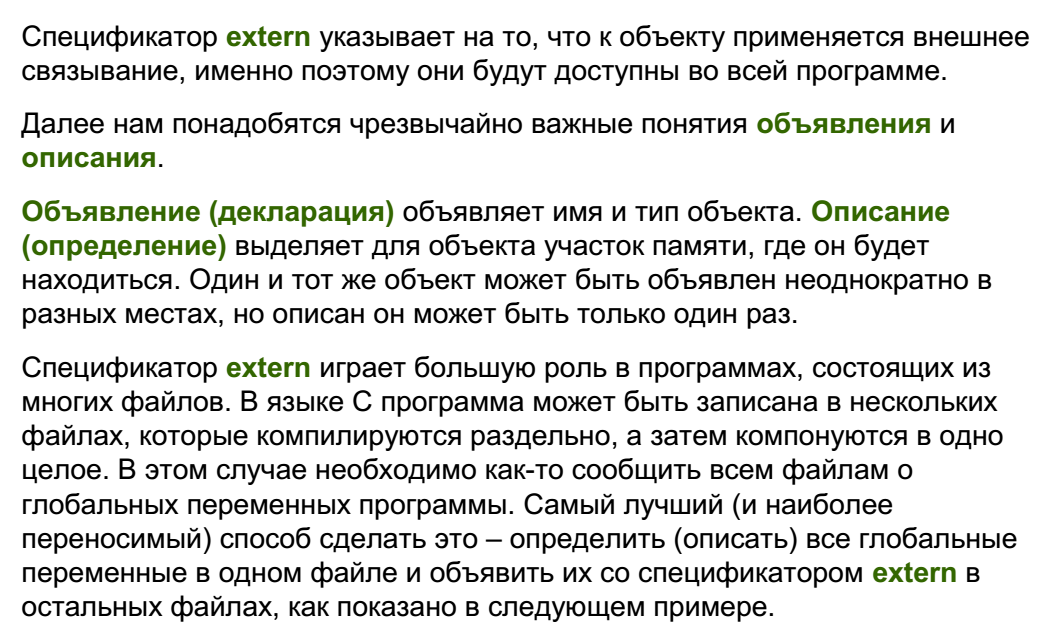
\includegraphics[scale=0.4]{images/lec02-pic10.png}
\end{figure}
\end{frame}

\begin{frame}{Спецификатор extern}
\begin{figure}[h]
\centering
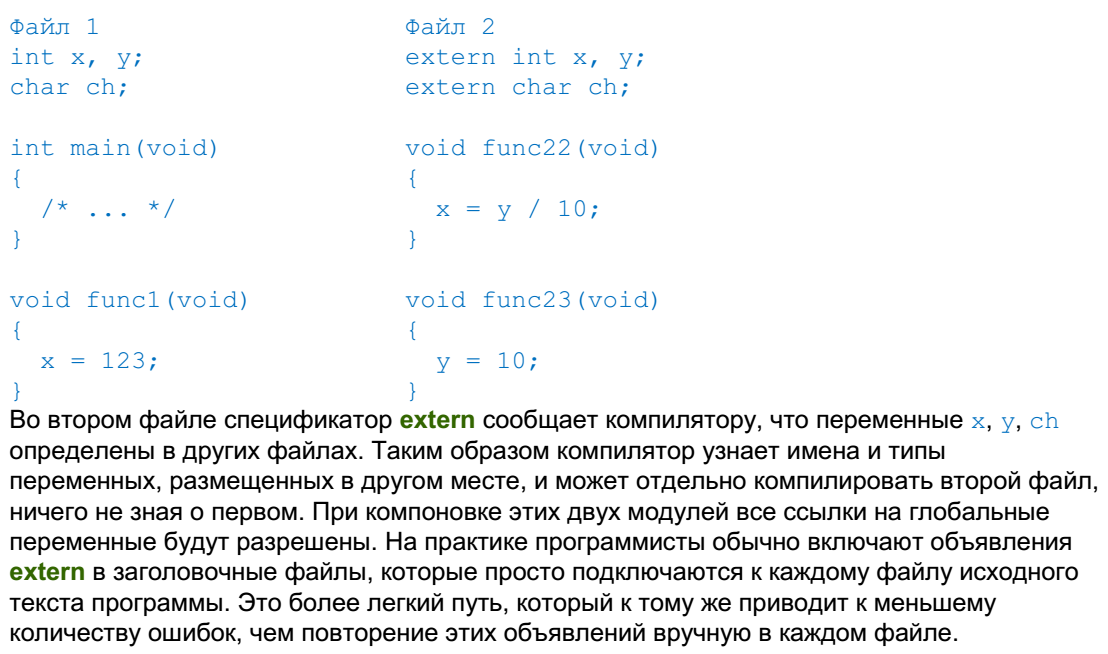
\includegraphics[scale=0.4]{images/lec02-pic11.png}
\end{figure}
\end{frame}

\begin{frame}{Спецификатор static}
\begin{figure}[h]
\centering
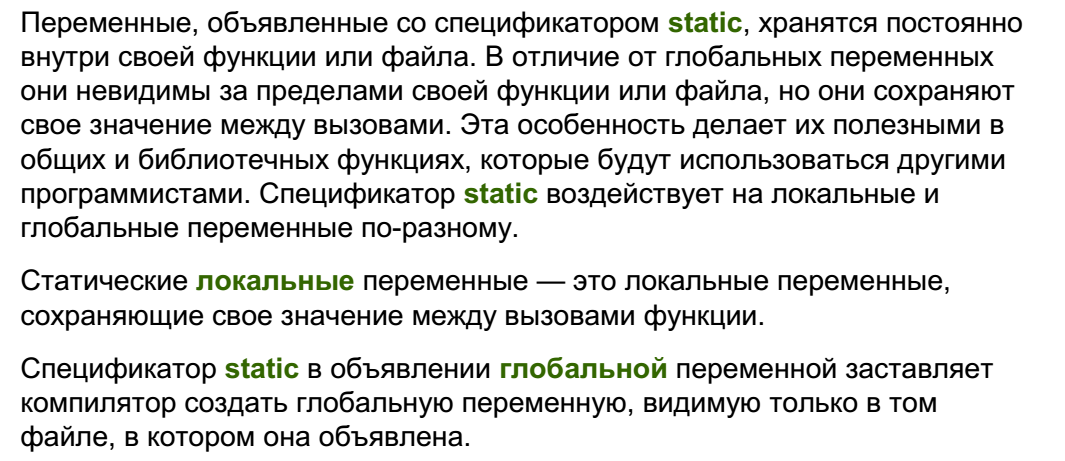
\includegraphics[scale=0.4]{images/lec02-pic12.png}
\end{figure}
\end{frame}

\begin{frame}{Спецификатор resgister}
\begin{figure}[h]
\centering
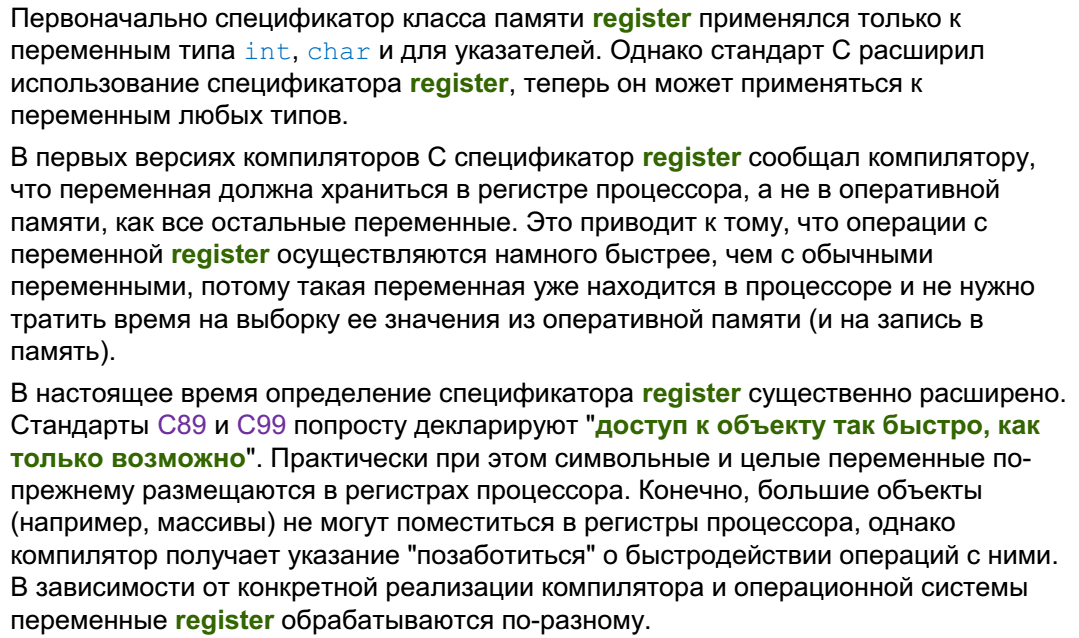
\includegraphics[scale=0.4]{images/lec02-pic13.png}
\end{figure}
\end{frame}

\section{Условный оператор}

\begin{frame}{Условный оператор if}
\begin{figure}[h]
\centering
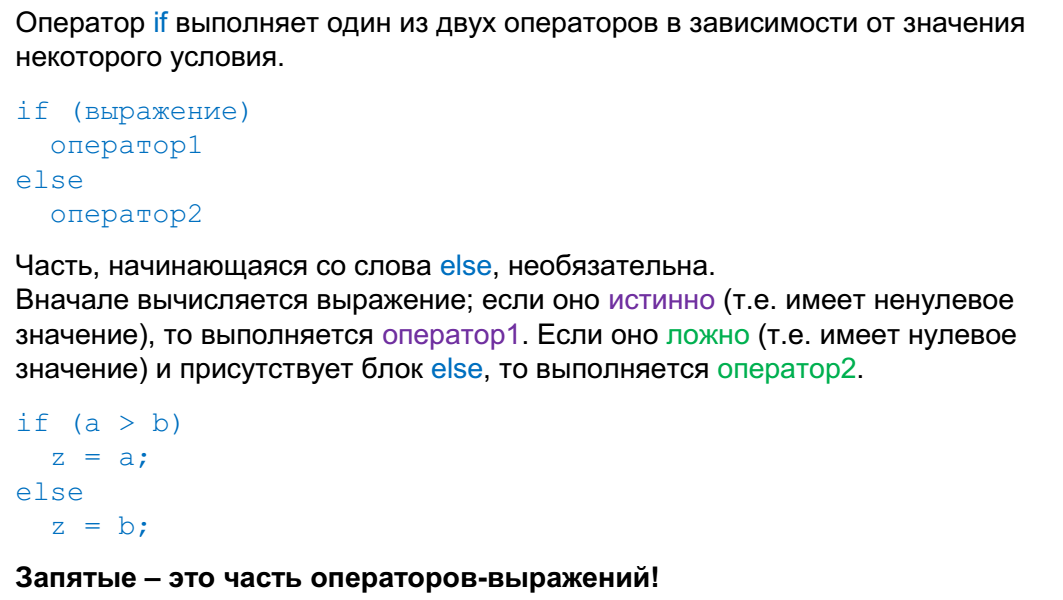
\includegraphics[scale=0.4]{images/lec02-pic14.png}
\end{figure}
\end{frame}

\section{Оператор выбора}

\begin{frame}{Оператор выбора switch}
\begin{figure}[h]
\centering
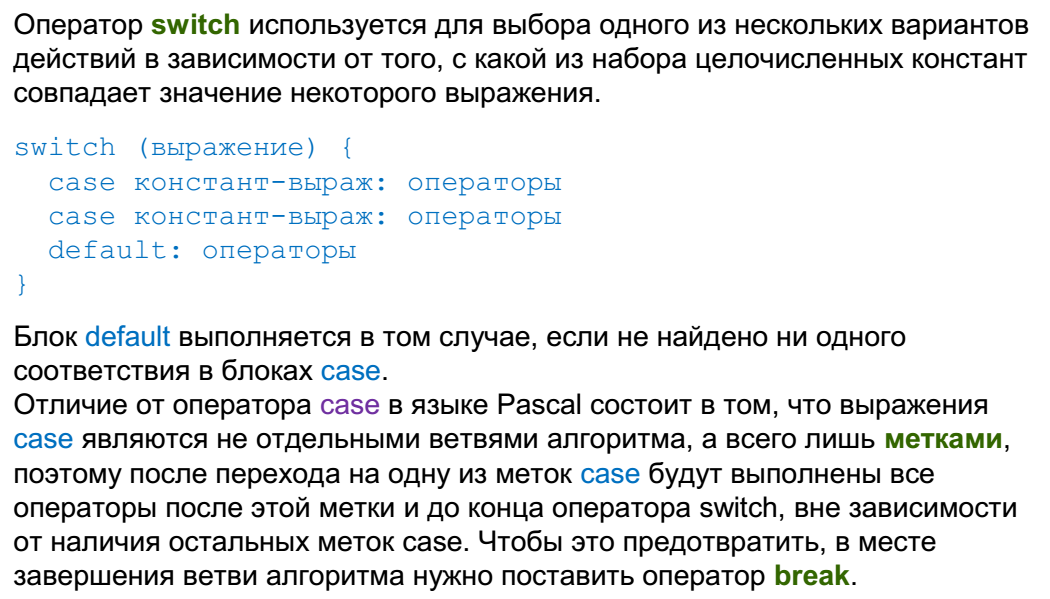
\includegraphics[scale=0.4]{images/lec02-pic15.png}
\end{figure}
\end{frame}

\section{Операторы циклов}

\begin{frame}{Оператор цикла while}
\begin{figure}[h]
\centering
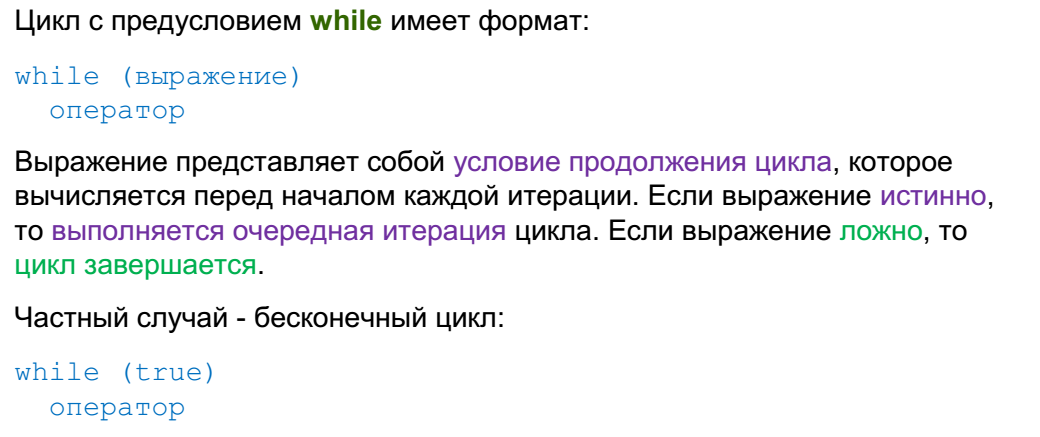
\includegraphics[scale=0.4]{images/lec02-pic16.png}
\end{figure}
\end{frame}

\begin{frame}{Оператор цикла do-while}
\begin{figure}[h]
\centering
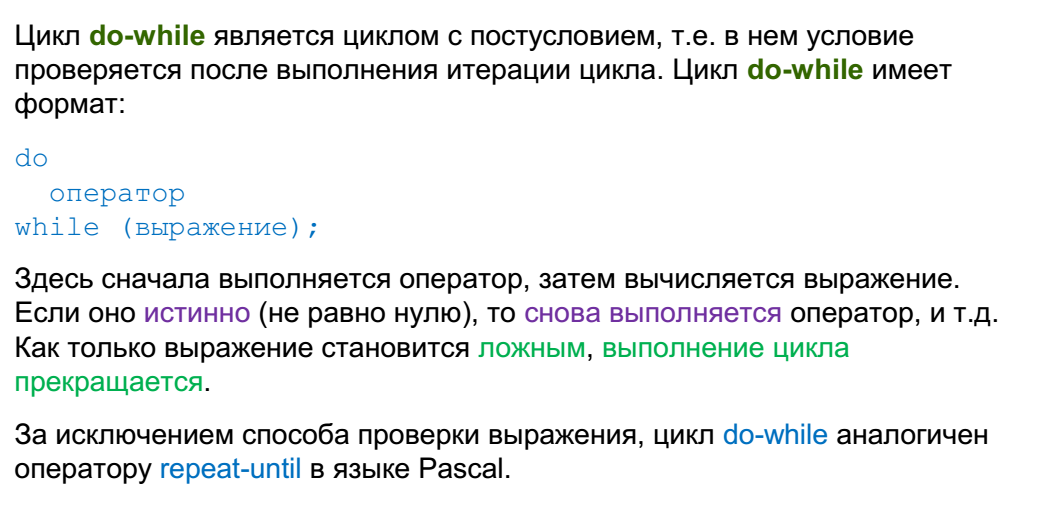
\includegraphics[scale=0.4]{images/lec02-pic17.png}
\end{figure}
\end{frame}

\begin{frame}{Оператор цикла for}
\begin{figure}[h]
\centering
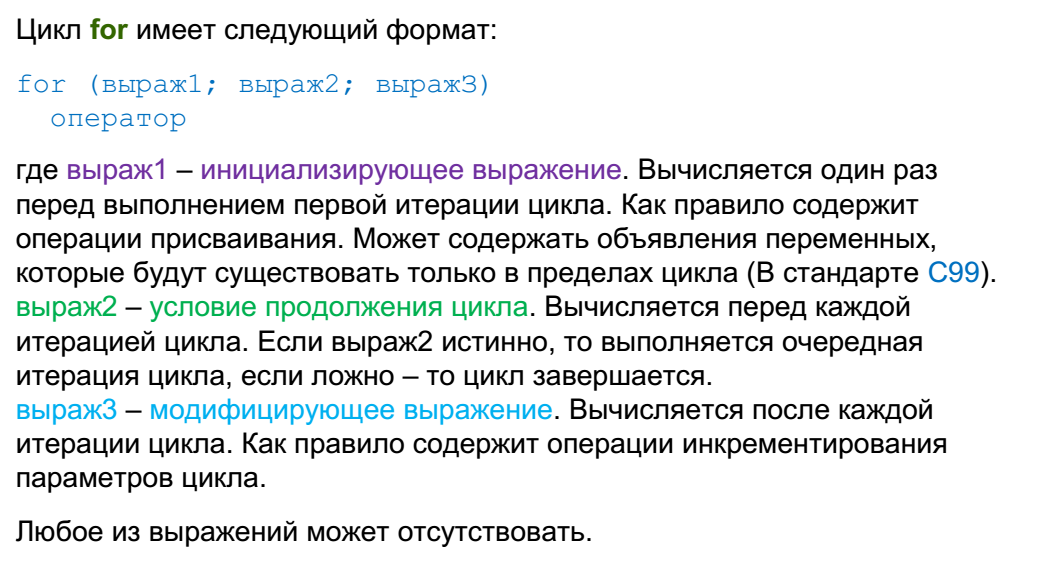
\includegraphics[scale=0.4]{images/lec02-pic18.png}
\end{figure}
\end{frame}

\begin{frame}{Оператор цикла for}
\begin{figure}[h]
\centering
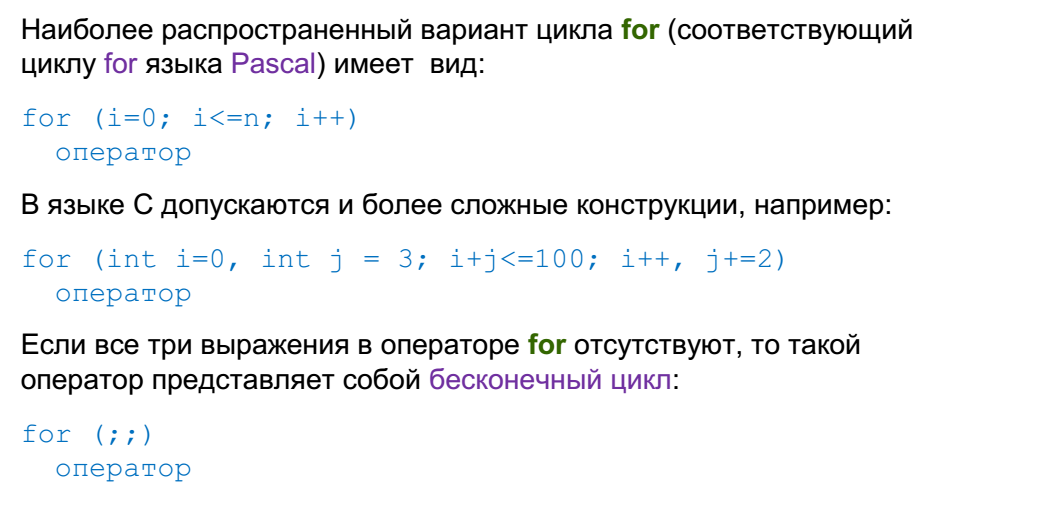
\includegraphics[scale=0.4]{images/lec02-pic19.png}
\end{figure}
\end{frame}

\section{Операторы break, continue, return, goto}

\begin{frame}{Метки. Оператор goto}
\begin{figure}[h]
\centering
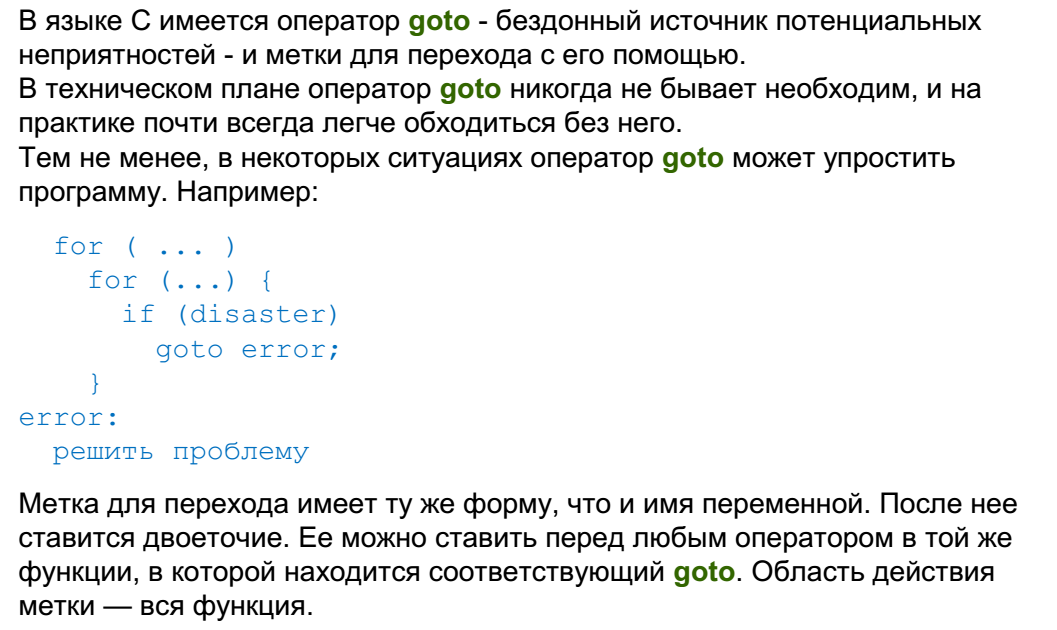
\includegraphics[scale=0.4]{images/lec02-pic20.png}
\end{figure}
\end{frame}

\begin{frame}{Операторы break и continue}
\begin{figure}[h]
\centering
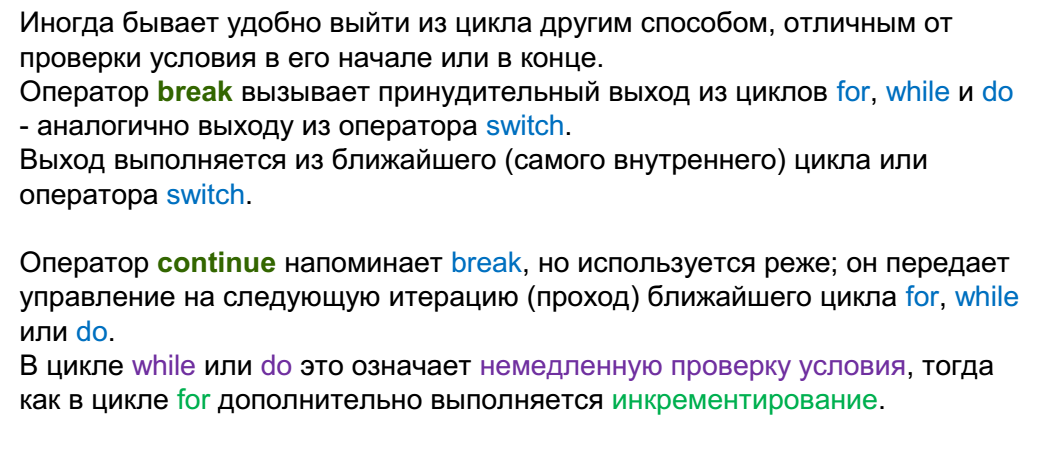
\includegraphics[scale=0.4]{images/lec02-pic21.png}
\end{figure}
\end{frame}

\begin{frame}{Оператор возврата из функции return}
\begin{figure}[h]
\centering
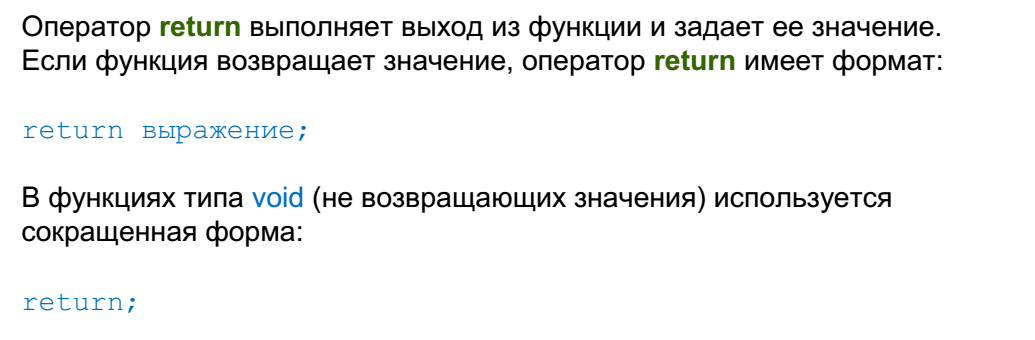
\includegraphics[scale=0.4]{images/lec02-pic22.png}
\end{figure}
\end{frame}

\section{Функции ввода-вывода}

\begin{frame}{Функции ввода/вывода на консоль}
\begin{figure}[h]
\centering
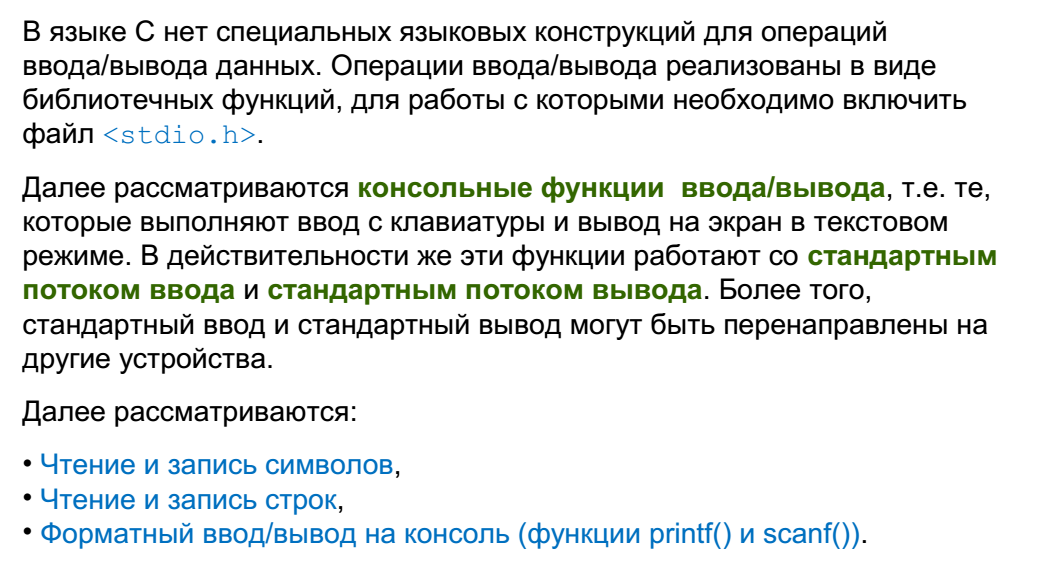
\includegraphics[scale=0.4]{images/lec02-pic23.png}
\end{figure}
\end{frame}

\begin{frame}{Чтение и запись символов}
\begin{figure}[h]
\centering
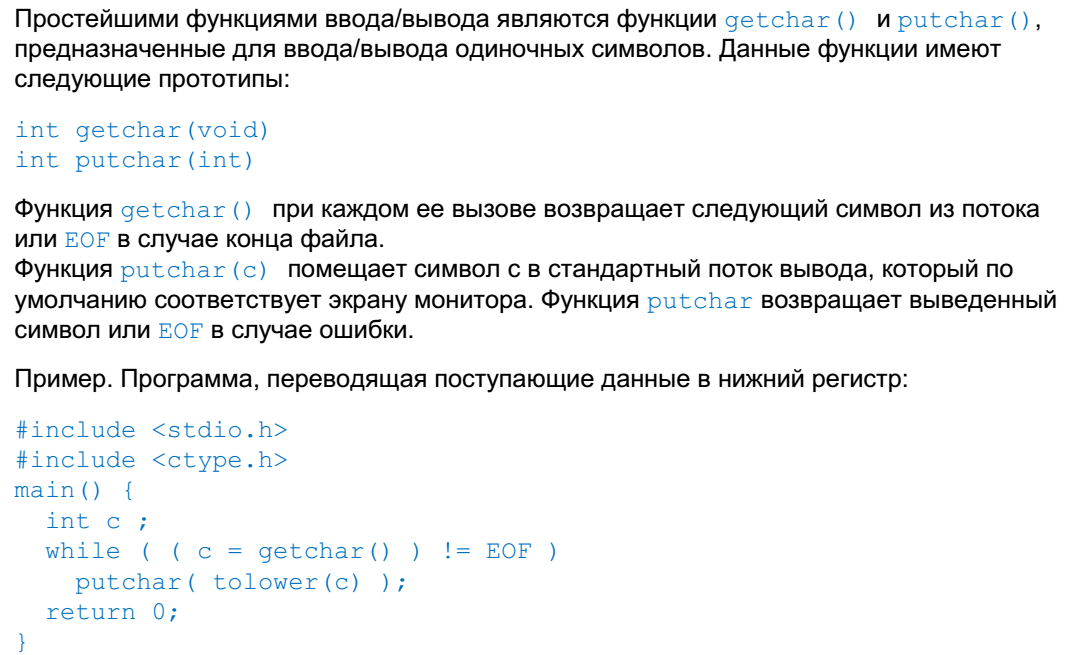
\includegraphics[scale=0.4]{images/lec02-pic24.png}
\end{figure}
\end{frame}

\begin{frame}{Чтение и запись строк}
\begin{figure}[h]
\centering
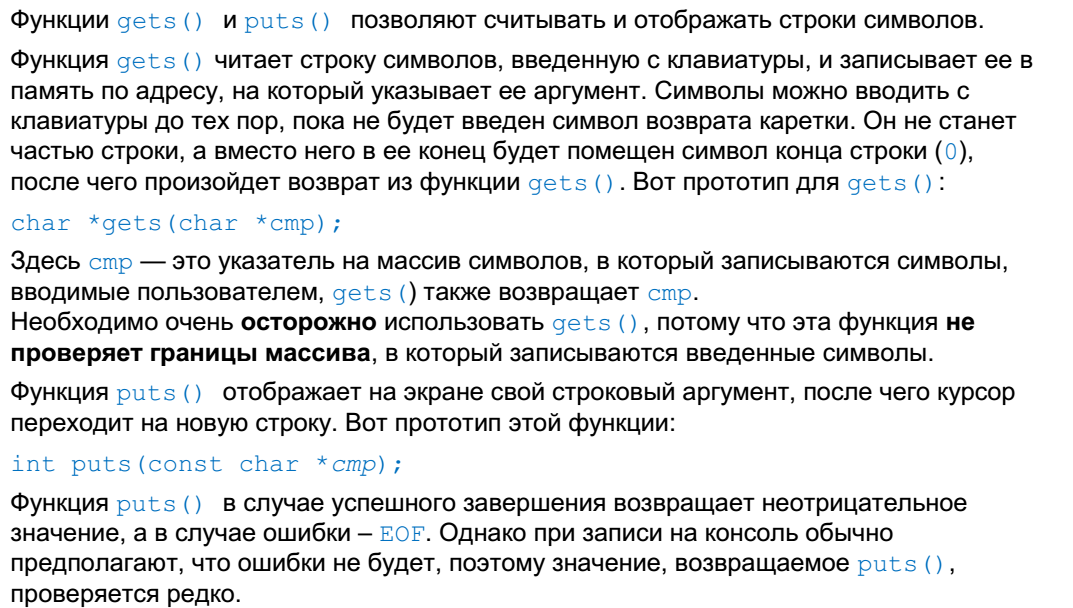
\includegraphics[scale=0.4]{images/lec02-pic25.png}
\end{figure}
\end{frame}

\begin{frame}{Форматный ввод/вывод на консоль}
\begin{figure}[h]
\centering
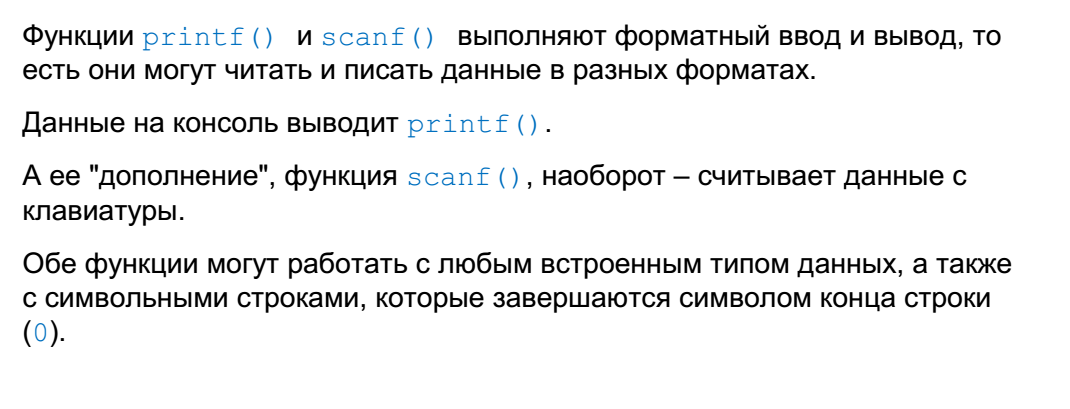
\includegraphics[scale=0.4]{images/lec02-pic26.png}
\end{figure}
\end{frame}

\begin{frame}{Функция printf()}
\begin{figure}[h]
\centering
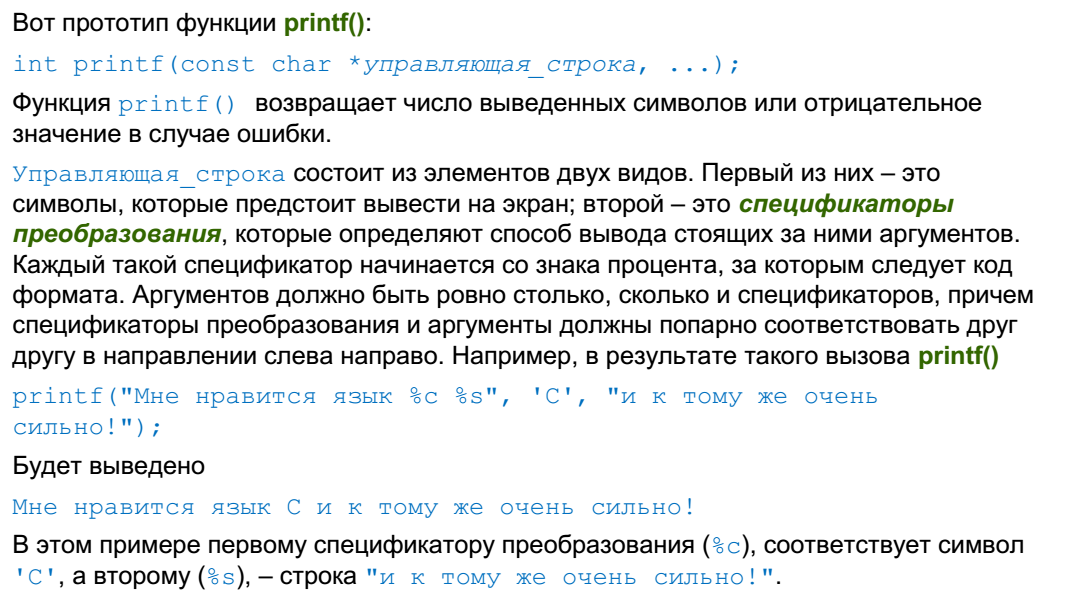
\includegraphics[scale=0.4]{images/lec02-pic27.png}
\end{figure}
\end{frame}

\begin{frame}{Спецификаторы преобразования для функции printf()}
\begin{figure}[h]
\centering
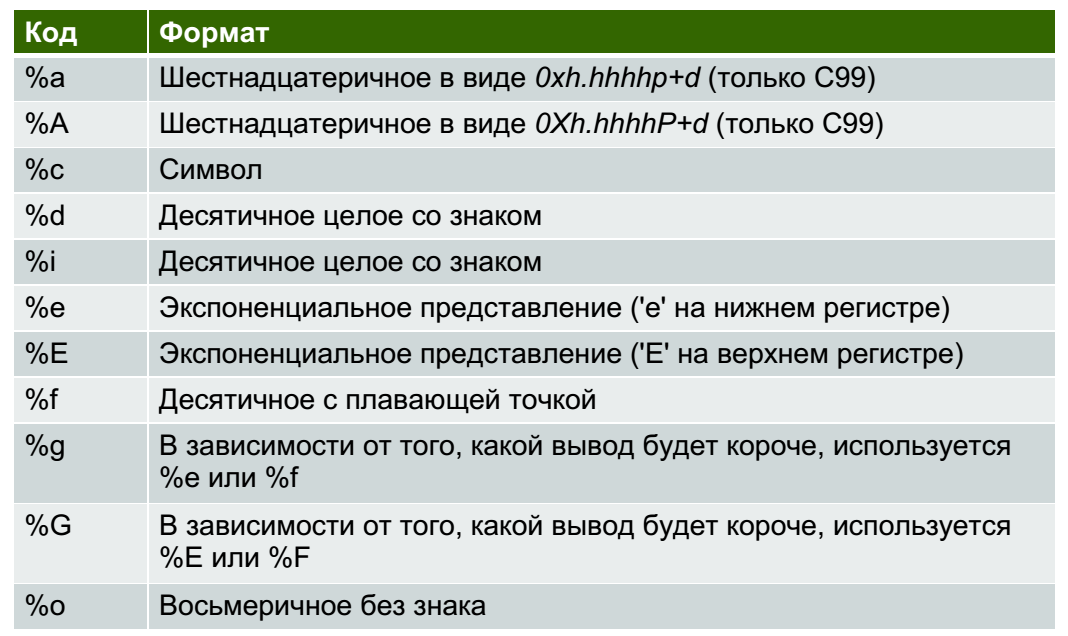
\includegraphics[scale=0.4]{images/lec02-pic28.png}
\end{figure}
\end{frame}

\begin{frame}{Спецификаторы преобразования для функции printf()}
\begin{figure}[h]
\centering
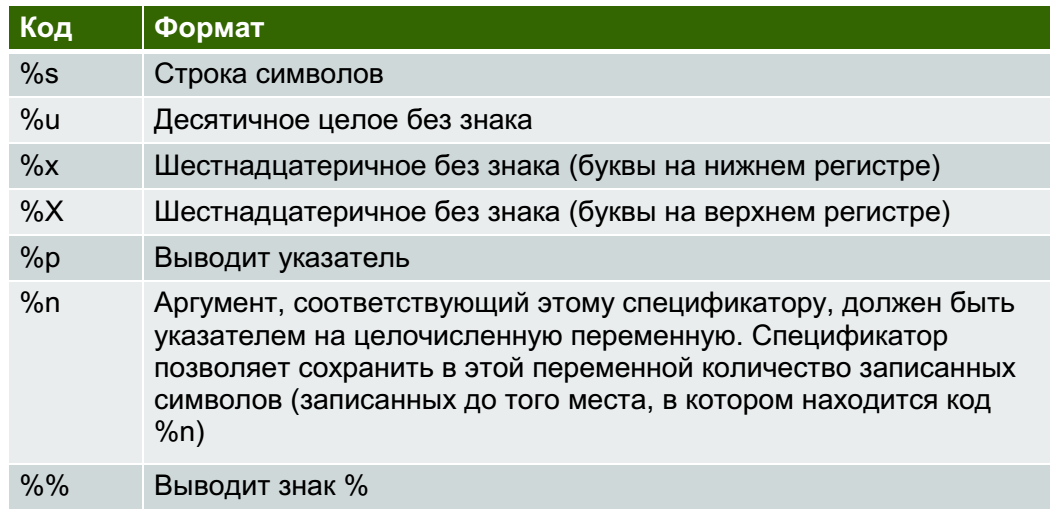
\includegraphics[scale=0.4]{images/lec02-pic29.png}
\end{figure}
\end{frame}

\begin{frame}{Модификаторы формата функции printf()}
\begin{figure}[h]
\centering
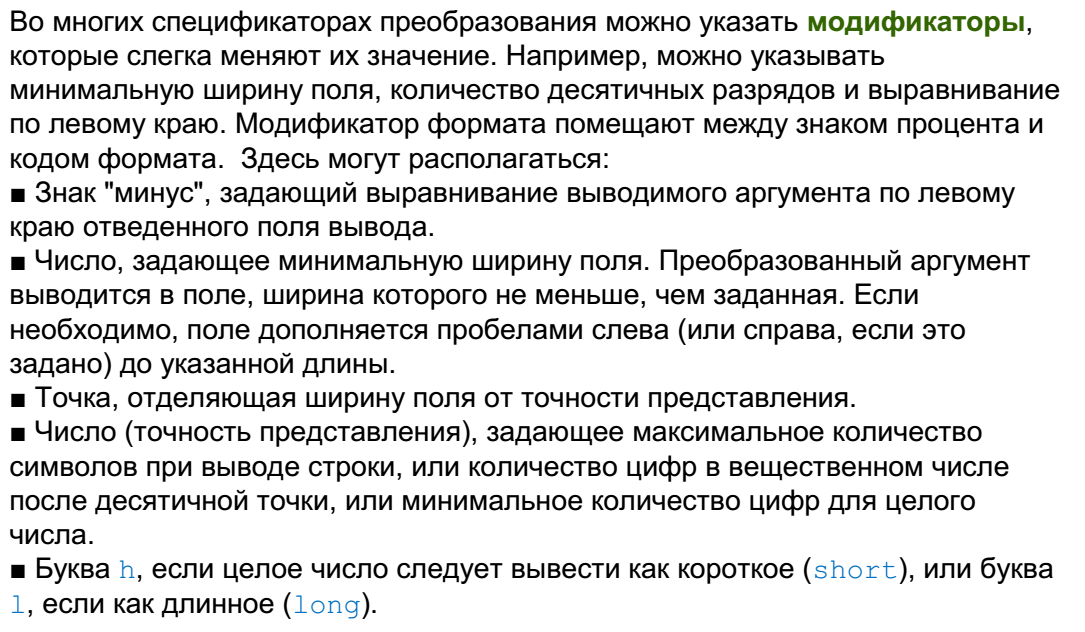
\includegraphics[scale=0.4]{images/lec02-pic30.png}
\end{figure}
\end{frame}

\begin{frame}{Пример. Модификаторы минимальной ширины поля}
\begin{figure}[h]
\centering
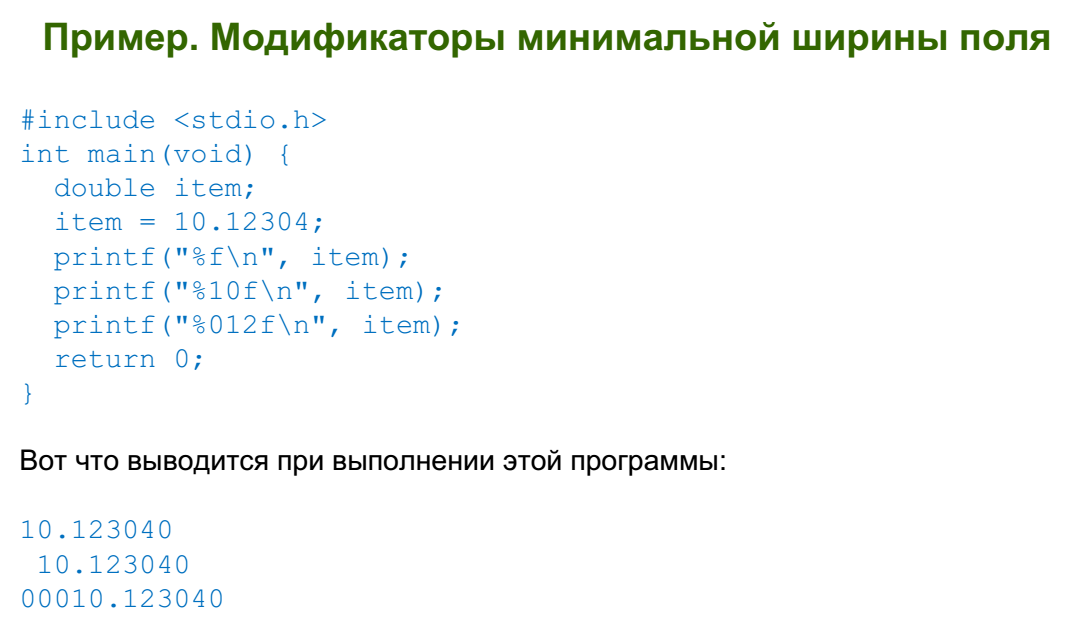
\includegraphics[scale=0.4]{images/lec02-pic31.png}
\end{figure}
\end{frame}

\begin{frame}{Пример. Выравнивание вывода}
\begin{figure}[h]
\centering
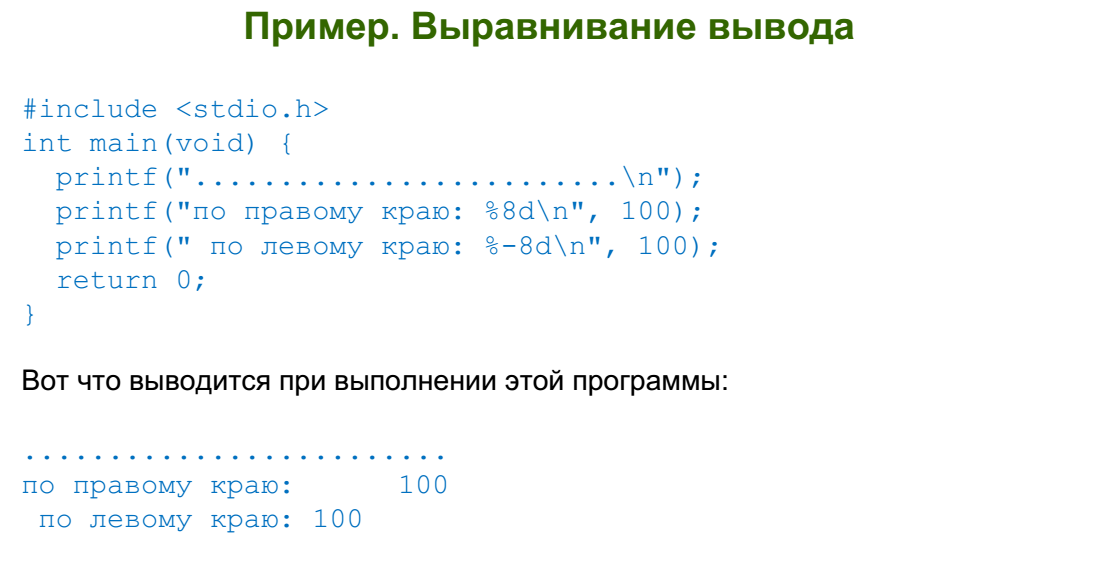
\includegraphics[scale=0.4]{images/lec02-pic32.png}
\end{figure}
\end{frame}

\begin{frame}{Функция scanf()}
\begin{figure}[h]
\centering
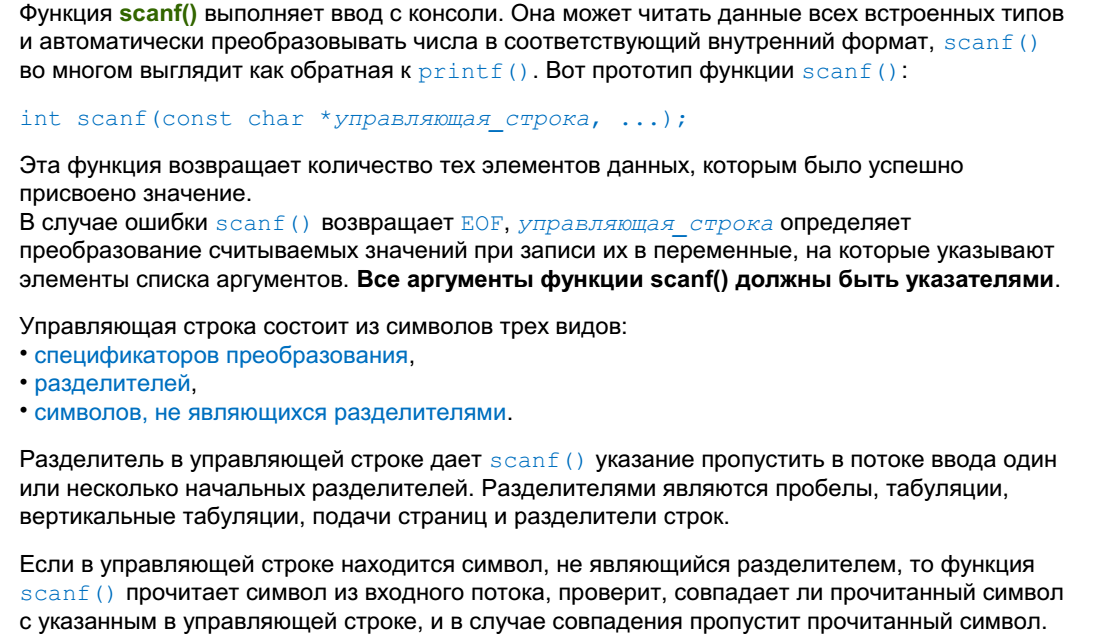
\includegraphics[scale=0.4]{images/lec02-pic33.png}
\end{figure}
\end{frame}

\begin{frame}{Спецификаторы преобразования для функции scanf()}
\begin{figure}[h]
\centering
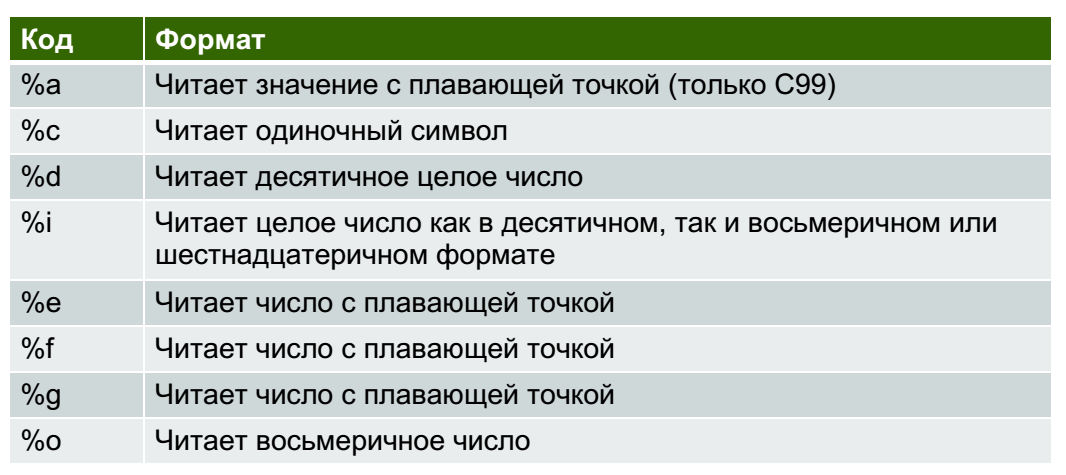
\includegraphics[scale=0.4]{images/lec02-pic34.png}
\end{figure}
\end{frame}

\begin{frame}{Спецификаторы преобразования для функции scanf()}
\begin{figure}[h]
\centering
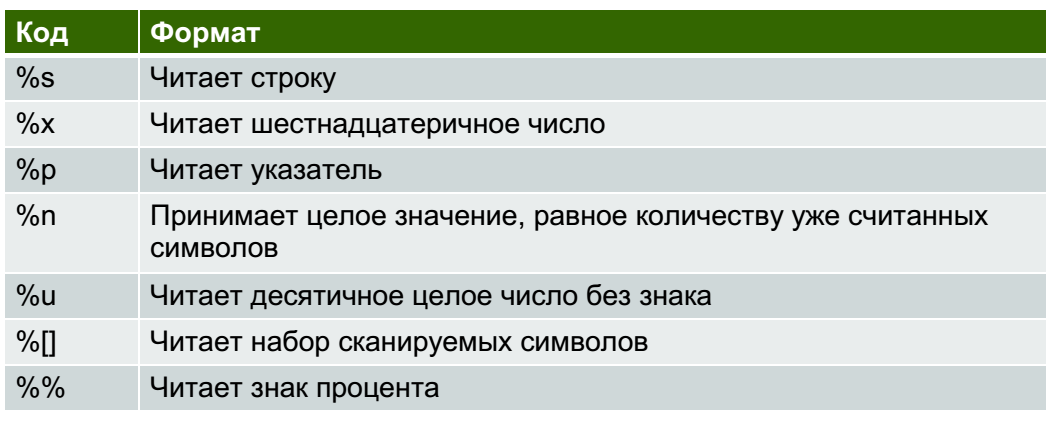
\includegraphics[scale=0.4]{images/lec02-pic35.png}
\end{figure}
\end{frame}

\begin{frame}{Примеры использования функции scanf()}
\begin{figure}[h]
\centering
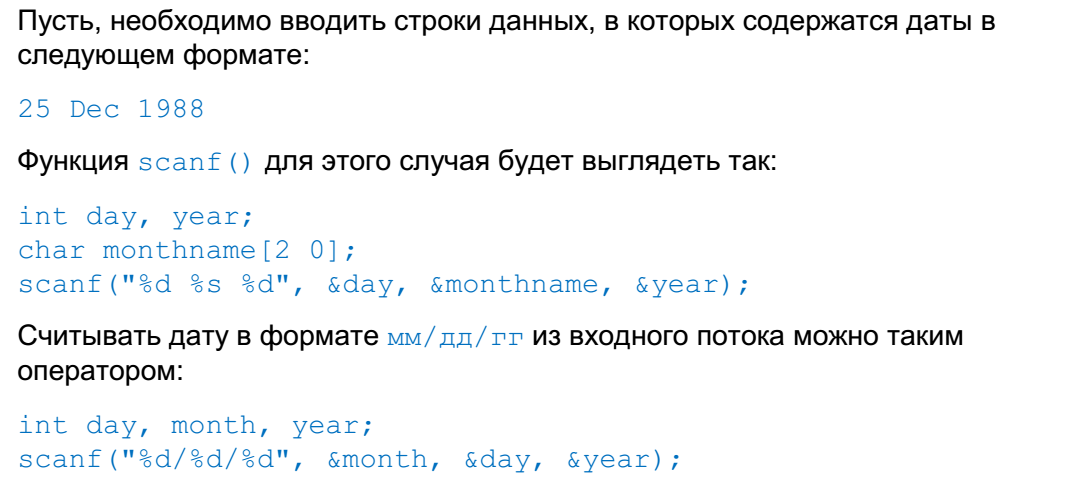
\includegraphics[scale=0.4]{images/lec02-pic36.png}
\end{figure}
\end{frame}

\end{document}
